\documentclass[11pt,preprint, authoryear]{elsarticle}

\usepackage{lmodern}
%%%% My spacing
\usepackage{setspace}
\setstretch{1.2}
\DeclareMathSizes{12}{14}{10}{10}

% Wrap around which gives all figures included the [H] command, or places it "here". This can be tedious to code in Rmarkdown.
\usepackage{float}
\let\origfigure\figure
\let\endorigfigure\endfigure
\renewenvironment{figure}[1][2] {
    \expandafter\origfigure\expandafter[H]
} {
    \endorigfigure
}

\let\origtable\table
\let\endorigtable\endtable
\renewenvironment{table}[1][2] {
    \expandafter\origtable\expandafter[H]
} {
    \endorigtable
}


\usepackage{ifxetex,ifluatex}
\usepackage{fixltx2e} % provides \textsubscript
\ifnum 0\ifxetex 1\fi\ifluatex 1\fi=0 % if pdftex
  \usepackage[T1]{fontenc}
  \usepackage[utf8]{inputenc}
\else % if luatex or xelatex
  \ifxetex
    \usepackage{mathspec}
    \usepackage{xltxtra,xunicode}
  \else
    \usepackage{fontspec}
  \fi
  \defaultfontfeatures{Mapping=tex-text,Scale=MatchLowercase}
  \newcommand{\euro}{€}
\fi

\usepackage{amssymb, amsmath, amsthm, amsfonts}

\def\bibsection{\section*{References}} %%% Make "References" appear before bibliography


\usepackage[round]{natbib}

\usepackage{longtable}
\usepackage[margin=2.3cm,bottom=2cm,top=2.5cm, includefoot]{geometry}
\usepackage{fancyhdr}
\usepackage[bottom, hang, flushmargin]{footmisc}
\usepackage{graphicx}
\numberwithin{equation}{section}
\numberwithin{figure}{section}
\numberwithin{table}{section}
\setlength{\parindent}{0cm}
\setlength{\parskip}{1.3ex plus 0.5ex minus 0.3ex}
\usepackage{textcomp}
\renewcommand{\headrulewidth}{0pt}

\usepackage{array}
\newcolumntype{x}[1]{>{\centering\arraybackslash\hspace{0pt}}p{#1}}

%%%%  Remove the "preprint submitted to" part. Don't worry about this either, it just looks better without it:
\makeatletter
\def\ps@pprintTitle{%
  \let\@oddhead\@empty
  \let\@evenhead\@empty
  \let\@oddfoot\@empty
  \let\@evenfoot\@oddfoot
}
\makeatother

 \def\tightlist{} % This allows for subbullets!

\usepackage{hyperref}
\hypersetup{breaklinks=true,
            bookmarks=true,
            colorlinks=true,
            citecolor=blue,
            urlcolor=blue,
            linkcolor=blue,
            pdfborder={0 0 0}}


% The following packages allow huxtable to work:
\usepackage{siunitx}
\usepackage{multirow}
\usepackage{hhline}
\usepackage{calc}
\usepackage{tabularx}
\usepackage{booktabs}
\usepackage{caption}


\newenvironment{columns}[1][]{}{}

\newenvironment{column}[1]{\begin{minipage}{#1}\ignorespaces}{%
\end{minipage}
\ifhmode\unskip\fi
\aftergroup\useignorespacesandallpars}

\def\useignorespacesandallpars#1\ignorespaces\fi{%
#1\fi\ignorespacesandallpars}

\makeatletter
\def\ignorespacesandallpars{%
  \@ifnextchar\par
    {\expandafter\ignorespacesandallpars\@gobble}%
    {}%
}
\makeatother

\newlength{\cslhangindent}
\setlength{\cslhangindent}{1.5em}
\newenvironment{CSLReferences}%
  {\setlength{\parindent}{0pt}%
  \everypar{\setlength{\hangindent}{\cslhangindent}}\ignorespaces}%
  {\par}


\urlstyle{same}  % don't use monospace font for urls
\setlength{\parindent}{0pt}
\setlength{\parskip}{6pt plus 2pt minus 1pt}
\setlength{\emergencystretch}{3em}  % prevent overfull lines
\setcounter{secnumdepth}{5}

%%% Use protect on footnotes to avoid problems with footnotes in titles
\let\rmarkdownfootnote\footnote%
\def\footnote{\protect\rmarkdownfootnote}
\IfFileExists{upquote.sty}{\usepackage{upquote}}{}

%%% Include extra packages specified by user

%%% Hard setting column skips for reports - this ensures greater consistency and control over the length settings in the document.
%% page layout
%% paragraphs
\setlength{\baselineskip}{12pt plus 0pt minus 0pt}
\setlength{\parskip}{12pt plus 0pt minus 0pt}
\setlength{\parindent}{0pt plus 0pt minus 0pt}
%% floats
\setlength{\floatsep}{12pt plus 0 pt minus 0pt}
\setlength{\textfloatsep}{20pt plus 0pt minus 0pt}
\setlength{\intextsep}{14pt plus 0pt minus 0pt}
\setlength{\dbltextfloatsep}{20pt plus 0pt minus 0pt}
\setlength{\dblfloatsep}{14pt plus 0pt minus 0pt}
%% maths
\setlength{\abovedisplayskip}{12pt plus 0pt minus 0pt}
\setlength{\belowdisplayskip}{12pt plus 0pt minus 0pt}
%% lists
\setlength{\topsep}{10pt plus 0pt minus 0pt}
\setlength{\partopsep}{3pt plus 0pt minus 0pt}
\setlength{\itemsep}{5pt plus 0pt minus 0pt}
\setlength{\labelsep}{8mm plus 0mm minus 0mm}
\setlength{\parsep}{\the\parskip}
\setlength{\listparindent}{\the\parindent}
%% verbatim
\setlength{\fboxsep}{5pt plus 0pt minus 0pt}



\begin{document}



\begin{frontmatter}  %

\title{How do oil price changes impact economic variables in the period
1990 to 2017: A Replication of the Cologni \& Manera paper}

% Set to FALSE if wanting to remove title (for submission)




\author[Add1]{Harriet Catherine Laing}
\ead{21617023@sun.ac.za}





\address[Add1]{Stellenbosch University, Stellenbosch, South Africa}



\vspace{1cm}





\vspace{0.5cm}

\end{frontmatter}



%________________________
% Header and Footers
%%%%%%%%%%%%%%%%%%%%%%%%%%%%%%%%%
\pagestyle{fancy}
\chead{}
\rhead{}
\lfoot{}
\rfoot{\footnotesize Page \thepage}
\lhead{}
%\rfoot{\footnotesize Page \thepage } % "e.g. Page 2"
\cfoot{}

%\setlength\headheight{30pt}
%%%%%%%%%%%%%%%%%%%%%%%%%%%%%%%%%
%________________________

\headsep 35pt % So that header does not go over title




\hypertarget{introduction}{%
\section{\texorpdfstring{Introduction
\label{Introduction}}{Introduction }}\label{introduction}}

To replicate the study by Cologni \& Manera, the same methodology and
structural cointegrated VAR model was used. This paper investigates
whether the findings from Cologni \& Manera hold after 2003 in the
United States, as the economic impact of a rise in oil prices during the
period 1990 to 2017 is analysed. The Cologni \& Manera paper sought to
find the impact of an increase in the world oil price on economic
variables and whether the response of central banks to a sudden oil
price shock reduced the impact thereof. However, the scope of this
replication is limited to the impulse response functions for each
variable.

This replication paper finds that\ldots is the optimal model for this
time period and \ldots{}

\hypertarget{background}{%
\section{Background}\label{background}}

Many economists regard increases in the oil price as a major cause of
asymmetries in the business cycle. Many studies have found a negative
impact on aggregate economic activity as a result of an increase in the
oil price (Hamilton, 1983). This issue became especially important to
economists following the world oil market highs in the early 2000s which
could lead to economic slowdowns in developed countries. The
hypothesised asymmetric relationship between oil prices and economic
activity was first hypothesised after the oil price collapse of 1986
which did not lead to an economic boom, which is what theoretically
should have been the case following the view that there existed an
inverse relationship between oil prices and the economy.

However, the channels through which an increase in the oil price impacts
economic variables remains unclear. There are many possible theoretical
explanations; some of which link to the effect of decreasing firms'
profits which may reduce capital spending and consumers' expectations
which causes them to consume more today, others link to the income
transfer between oil-importing countries and oil exporting countries
that shifts, and others link an increase in oil prices to the increases
in prices of related goods, thereby increasing inflation.

There is also, importantly, effects on economic variables that flow
indirectly from an increase in oil prices. Namely, that the monetary
authority responds to increase employment and ensure price stability
once an increase in oil prices threatens these two objectives. For
example, in the US, the Federal bank \ldots{} The role of monetary
policy may cause delayed impacts of an increase in oil prices on
economic variables.

Cologni \& Manera motivate their inclusion of exchange rates based on it
serving as a measurement of monetary policy because monetary authorities
may offset the short-term effect of a shock to the economy with the
exchange rate or they may target the exchange rate. The choice of time
period from 1980 to 2003 was because it was a volatile period for oil
prices and the authors sought to verify the role of exogenous shocks at
this time. Cologni \& Manera impose short-run and long-run restrictions
on the model based on economic theory. Thereafter, cointegration
analysis is conducted on the long-run model, in other words, the VAR
system, and the lags are selected.

For our purposes, the imposition of both the long-run and short-run
restrictions was contrained by the capabilities of the coding software
used. Therefore, we imposed only the short-run restrictions. Moreover,
the inclusion of the exchange rate in the model is challenged on the
grounds that after the 2008 financial crisis which is included in our
period of analysis, interest rates were close to the lower bound which
undermined the Federal Bank's ability to target the exchange rate
(Amador et al, 2017). Moreover, an exchange rate is generally affected
indirectly from a change in interest rates, which therefore would be
captured in interest rates, rendering exchange rates in the model
specification redundant. As stated in Cologni \& Manera (2006), in order
to obtain a more parsimonious result, a visual representation of the
cointegrating vectors if two were identified by the Johansen test and
motivated by economic theory could be analysed. If the cointegrating
vectors looked to be trending, then include. But could motivate on
economic reasoning.

\hypertarget{replication-methodology-results}{%
\section{Replication methodology \&
results}\label{replication-methodology-results}}

\hypertarget{finding-the-data}{%
\subsection{Finding the data}\label{finding-the-data}}

The data for this replication was sourced where possible from the IMF to
be as similar to Cologni \& Manera's method as possible. However, for
the interest rate and exchange rate we sourced the data from Board of
Governors of the Federal Reserve System and for inflation the data was
obtained from the US Bureau of Labor Statistics. Firstly, all the data
was converted into quarterly data. The time period available to
reproduce the results of the paper was constrained by the availability
of world oil price and monetary aggregate data. For the world oil price,
data was only available from 1990, and for the monetary aggregate, data
was only available up until 2017. Therefore, our time period was
constrained due to data availability. In the Cologni \& Manera (2006)
paper, predominantly seasonally-adjusted data was used but due to
constraints on availability of data, for this replication I used a
combination of seasonally-adjusted and non-seasonally-adjusted data.

\begin{longtable}[]{@{}
  >{\raggedright\arraybackslash}p{(\columnwidth - 4\tabcolsep) * \real{0.2035}}
  >{\centering\arraybackslash}p{(\columnwidth - 4\tabcolsep) * \real{0.3717}}
  >{\centering\arraybackslash}p{(\columnwidth - 4\tabcolsep) * \real{0.4248}}@{}}
\toprule
\begin{minipage}[b]{\linewidth}\raggedright
Economic variable
\end{minipage} & \begin{minipage}[b]{\linewidth}\centering
Cologni \& Manera (all IMF)
\end{minipage} & \begin{minipage}[b]{\linewidth}\centering
Replication paper
\end{minipage} \\
\midrule
\endhead
Interest Rate & Federal Funds rate (\% per annum) & Federal Funds
Effective rate (\% per month) \\
Inflation & Consumer price index (index number) & Consumer price index
(1982-1984=100) \\
Real GDP & Real GDP (constant prices 1995) (billions) & Real GDP
(constant prices 1995) (billions) (IMF) \\
Monetary Aggregate & Money M1 (billions) & Money M1 (billions) (IMF) \\
Exchange Rate & US dollars (per SDR) & US dollars (millions) \\
World Oil Price & International average price (Brent dated) & US dollars
per barrel (IMF) \\
\bottomrule
\end{longtable}

Thereafter, all of the quarterly time series variables were transformed
in logarithms, except for the interest rate. As in the paper, Augmented
Dickey Fuller tests were run on all the time series variables. Findings
at the 1\% confidence interval were that are all variables were
non-stationary and were integrated of order 1, except for the monetary
aggregate which was found to be integrated of order 2. The results in
this replication for the Augmented Dickey Fuller tests differed only
from the paper regarding the integration order of inflation, which was
found to be integrated of order 1 by Cologni \& Manera. This difference
from the paper dictated that only the monetary aggregate be transformed
by subtracting inflation to become the real monetary aggregate (by
taking the difference between the logarithm of monetary aggregate and
the logarithm of inflation), and the transformation for inflation was
not followed. This is because for finding cointegrating relationships,
the time series variables must be integrated of order 1.

\begin{center}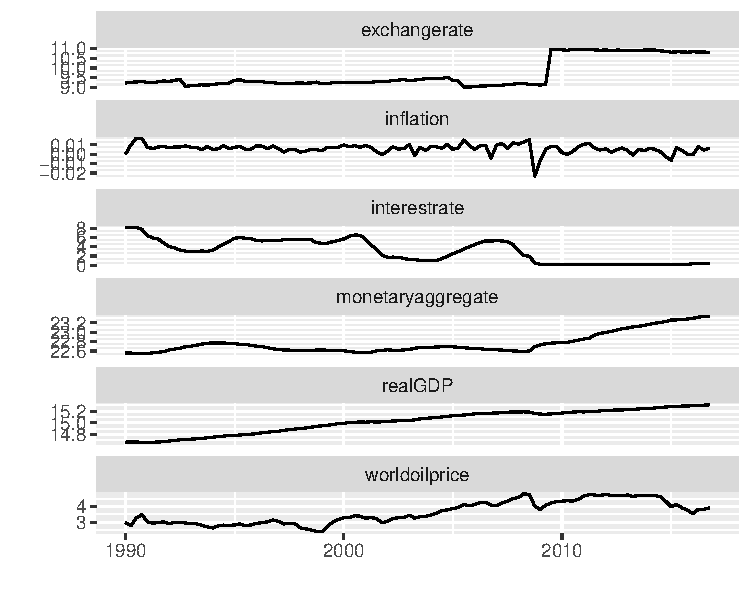
\includegraphics{README_files/figure-latex/unnamed-chunk-1-1} \end{center}

We then construct our VAR model and estimate the number of lags to be
included. According to the paper, the lag max is set to 4 and the AIC
lag selection criteria is used. The VAR model in the replication was
found to have 4 lags and accounted for a time trend, as is done in the
paper. We order our VAR system in the same way as the short run
restrictions matrix in the paper: monetary aggregate, interest rate,
real GDP, inflation, exchange rate and world oil price. Cologni \&
Manera find that the number of lags should be 2. As can be seen in
Figure 1, there is clearly a lot of persistence after the financial
crisis. Exchange rates for the US had a stark level increase around this
water-shed event and interest rates were set close to zero to try and
stimulate the economy, where they have remained fairly constant since
this monetary policy adjustment. Similarly, we can note real GDP has
diminished its upward trajectory path slightly since 2008. Therefore, it
is likely the difference in the optimal lags between this replication
and the Cologni \& Manera paper arises from the different time periods
used, as Cologni \& Manera's time period ends before the financial
crisis.

For a VAR model, we use the lag of 4. For the VECM model, we use the lag
of 3 because a VECM model has a difference term.

Now we can see long-run trends in the time series variables, but wish to
now see if there exists any cointegrating relationships. We test this
using the Johansen test, namely the eigenvalue test and the trace test.
For the eigenvalue test, we find we cannot reject the null hypothesis
that the number of cointegrating relationships is between 0 and 1 at the
5\% confidence interval where our critical value is smaller than the
test statistic, however, only marginally (37.26 estimated value
\textless{} 37.52 critical value). For the trace test, we find that we
cannot reject the null hypothesis that the number of cointegrating
relationships is between 1 and 2. Therefore, because the rejection of
the null hypothesis in the eigenvalue test is incredibly marginal, we
conclude from our estimates that there is likely two cointegrating
relationships. This is a divergence from the result as is found for the
US in Cologni \& Manera.

Cointegration analysis of the restricted system

We obtain the cointegrating vectors from the Johansen test and construct
a matrix is which each column is a cointegrating vector. Then we
multiply the VAR system by the cointegrating vector matrix to obtain the
error correction terms.

\hypertarget{restricted-var-system}{%
\section{Restricted VAR system}\label{restricted-var-system}}

The covariance matrix of residuals from the VAR system provides us with
an estimate of the contemporaneous effects of each variable.

Let us check which variables might be cointegrated, by regressing them
on each other and checking if the residuals are stationary or not

monetaryaggregate, interestrate, realGDP, inflation, exchangerate,
worldoilprice

\begin{verbatim}
## 
## Call:
## lm(formula = worldoilprice ~ interestrate, data = cointanalysisVAR)
## 
## Residuals:
##      Min       1Q   Median       3Q      Max 
## -0.94266 -0.47859 -0.09981  0.50308  1.15148 
## 
## Coefficients:
##              Estimate Std. Error t value Pr(>|t|)    
## (Intercept)   4.18258    0.08474  49.359  < 2e-16 ***
## interestrate -0.18810    0.02172  -8.661 5.72e-14 ***
## ---
## Signif. codes:  0 '***' 0.001 '**' 0.01 '*' 0.05 '.' 0.1 ' ' 1
## 
## Residual standard error: 0.5513 on 106 degrees of freedom
## Multiple R-squared:  0.4144, Adjusted R-squared:  0.4089 
## F-statistic: 75.01 on 1 and 106 DF,  p-value: 5.718e-14
\end{verbatim}

\begin{verbatim}
## 
## ############################################### 
## # Augmented Dickey-Fuller Test Unit Root Test # 
## ############################################### 
## 
## Test regression none 
## 
## 
## Call:
## lm(formula = z.diff ~ z.lag.1 - 1 + z.diff.lag)
## 
## Residuals:
##      Min       1Q   Median       3Q      Max 
## -0.84167 -0.08570  0.01493  0.10515  0.33617 
## 
## Coefficients:
##             Estimate Std. Error t value Pr(>|t|)    
## z.lag.1     -0.09937    0.03340  -2.975  0.00369 ** 
## z.diff.lag1  0.40830    0.09193   4.441 2.35e-05 ***
## z.diff.lag2 -0.08156    0.09961  -0.819  0.41486    
## z.diff.lag3  0.19250    0.09558   2.014  0.04674 *  
## z.diff.lag4  0.06950    0.09326   0.745  0.45791    
## ---
## Signif. codes:  0 '***' 0.001 '**' 0.01 '*' 0.05 '.' 0.1 ' ' 1
## 
## Residual standard error: 0.1663 on 98 degrees of freedom
## Multiple R-squared:  0.2295, Adjusted R-squared:  0.1902 
## F-statistic: 5.839 on 5 and 98 DF,  p-value: 9.195e-05
## 
## 
## Value of test-statistic is: -2.9751 
## 
## Critical values for test statistics: 
##       1pct  5pct 10pct
## tau1 -2.58 -1.95 -1.62
\end{verbatim}

At 1\%\ldots{} M \& IR not stationary, M\& G not, \& inf not, \&exch
not, \&oil not int rate and oil YES (yes) IR \& GDP yes (yes) IR \&
inflation yes (yes) IR \& exch rate yes (no) GDP \& exch no, \& infla
no, \%oil no infla \& exch no infla \& oil price yes (no) exh \& oil no

We want to set up our own VECM model

Let us set up the imposed restrictions in a matrix, known as B matrix in
the paper.

We want to find whether our restrictions are exogenous or not.

According to the paper, \(u_t=E_tB\) which means that we can recover the
short run error vector \(u_t\) from the long-run error we obtain from
our VAR system. We obtain the covariance matrix of residuals from our
VAR system and then mutiply that by our B matrix of short-run
restrictions and the transpose of the B matrix, because the paper states
that these are equivalent.

\begin{verbatim}
##                   MonetaryAggregate InterestRate      RealGDP Inflation
## MonetaryAggregate      0.0001328802   0.00000000 0.000000e+00  0.000000
## InterestRate           0.0000000000   0.07138726 0.000000e+00  0.000000
## RealGDP                0.0000000000   0.00000000 2.804883e-05  0.000000
## Inflation              0.0000000000   0.00000000 0.000000e+00  0.753182
## ExchangeRate           0.0000000000   0.00000000 0.000000e+00  0.000000
## WorldOilPrice          0.0000000000   0.00000000 0.000000e+00  0.000000
##                   ExchangeRate WorldOilPrice
## MonetaryAggregate   0.00000000    0.00000000
## InterestRate        0.00000000    0.00000000
## RealGDP             0.00000000    0.00000000
## Inflation           0.00000000    0.00000000
## ExchangeRate        0.01135468    0.00000000
## WorldOilPrice       0.00000000    0.02108534
\end{verbatim}

We then obtain a single entry for each row, which we can create our
short-run error vector from.

Comparison of cointegrating vectors

\begin{longtable}[]{@{}
  >{\raggedright\arraybackslash}p{(\columnwidth - 12\tabcolsep) * \real{0.2072}}
  >{\centering\arraybackslash}p{(\columnwidth - 12\tabcolsep) * \real{0.0901}}
  >{\centering\arraybackslash}p{(\columnwidth - 12\tabcolsep) * \real{0.1532}}
  >{\centering\arraybackslash}p{(\columnwidth - 12\tabcolsep) * \real{0.1351}}
  >{\centering\arraybackslash}p{(\columnwidth - 12\tabcolsep) * \real{0.0991}}
  >{\centering\arraybackslash}p{(\columnwidth - 12\tabcolsep) * \real{0.1351}}
  >{\centering\arraybackslash}p{(\columnwidth - 12\tabcolsep) * \real{0.1802}}@{}}
\toprule
\begin{minipage}[b]{\linewidth}\raggedright
\end{minipage} & \begin{minipage}[b]{\linewidth}\centering
Real GDP
\end{minipage} & \begin{minipage}[b]{\linewidth}\centering
World Oil Price
\end{minipage} & \begin{minipage}[b]{\linewidth}\centering
Interest Rate
\end{minipage} & \begin{minipage}[b]{\linewidth}\centering
Inflation
\end{minipage} & \begin{minipage}[b]{\linewidth}\centering
Exchange Rate
\end{minipage} & \begin{minipage}[b]{\linewidth}\centering
Monetary Aggregate
\end{minipage} \\
\midrule
\endhead
Cologni \& Manera & 1 & 0.16 & 0 & -26.019 & 0.218 & 0 \\
Cointegrating vector 1 & 1 & 0 & -0.170 & -0.017 & 0.616 & -0.375 \\
Cointegrating vector 2 & 0 & 1 & 1.606 & 0.0699 & -5.496 & 6.579 \\
\bottomrule
\end{longtable}

We need to find the SR error, which is equal to the LR error (ECT in the
VECM) multiplied by the SR restrictions (B matrix)

\begin{center}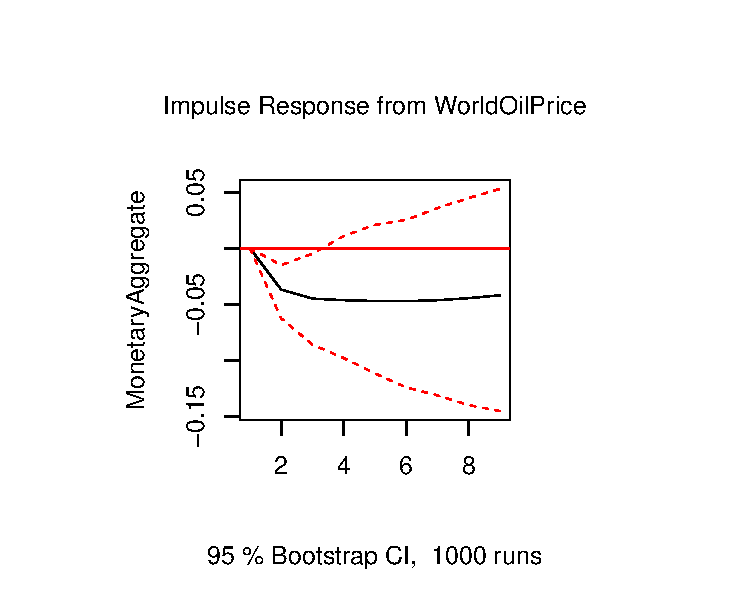
\includegraphics{README_files/figure-latex/unnamed-chunk-16-1} \end{center}

\begin{center}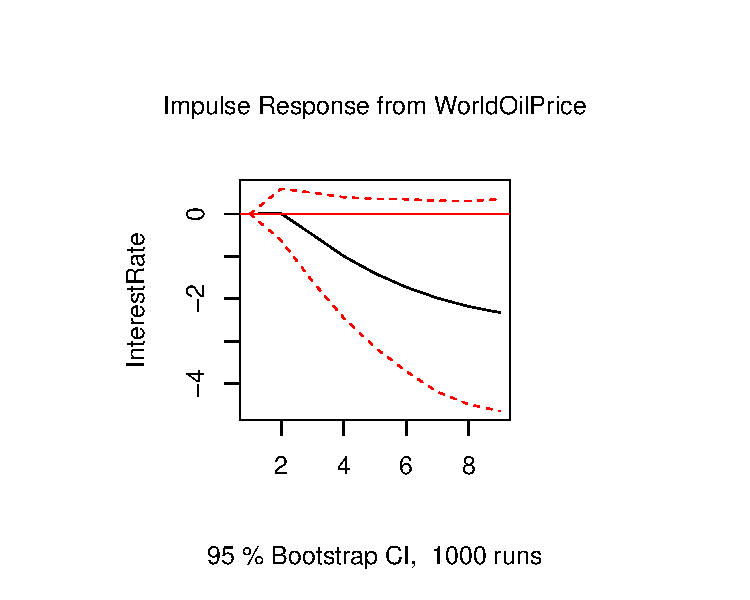
\includegraphics{README_files/figure-latex/unnamed-chunk-16-2} \end{center}

\begin{center}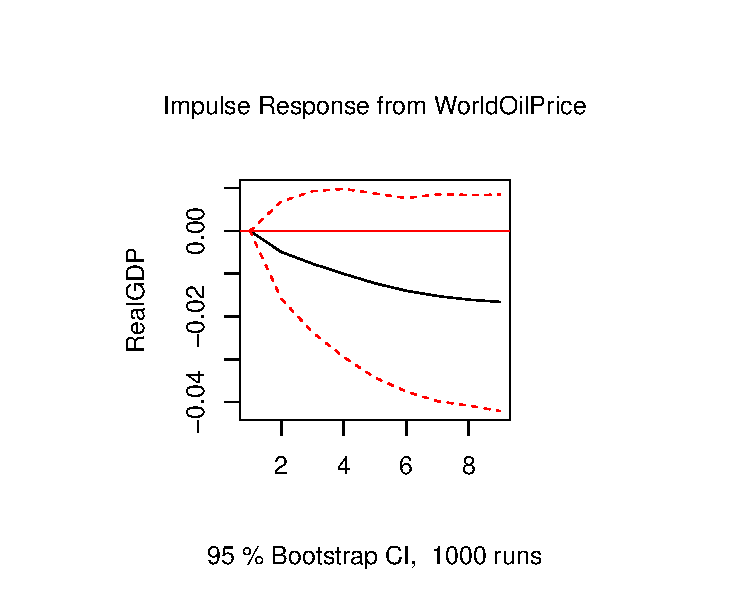
\includegraphics{README_files/figure-latex/unnamed-chunk-16-3} \end{center}

\begin{center}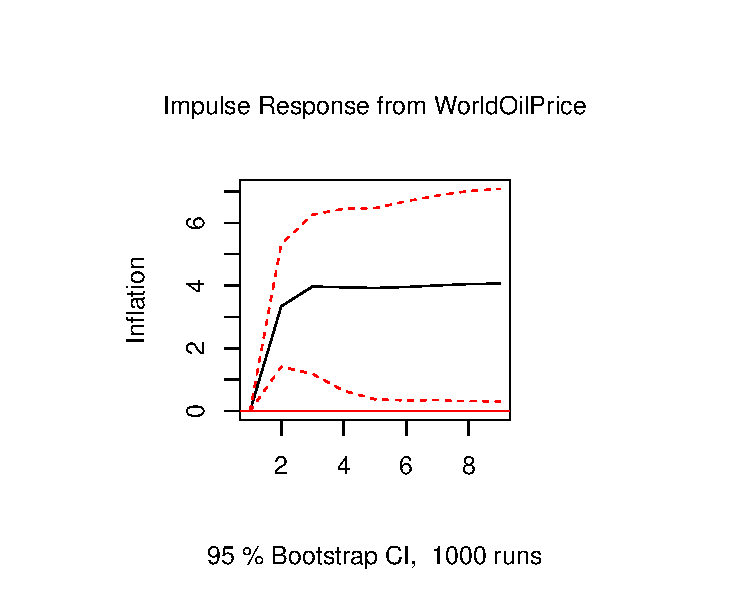
\includegraphics{README_files/figure-latex/unnamed-chunk-16-4} \end{center}

\begin{center}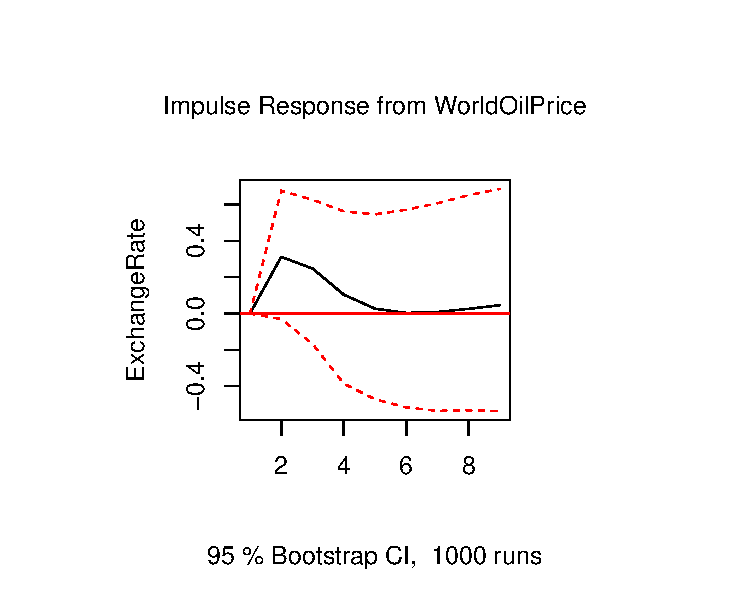
\includegraphics{README_files/figure-latex/unnamed-chunk-16-5} \end{center}

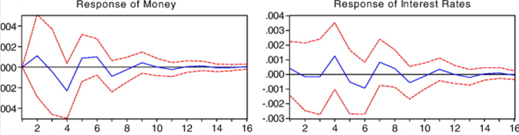
\includegraphics[width=\textwidth,height=0.4\textheight]{"C:/Users/Harriet/Documents/Econometrics/TimeSeriesProject/TimeSeriesProject/IRFs_firstcleearx.png"}

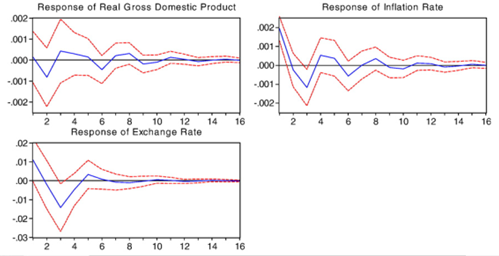
\includegraphics[width=\textwidth,height=0.4\textheight]{"C:/Users/Harriet/Documents/Econometrics/TimeSeriesProject/TimeSeriesProject/IRFs_secondx.png"}

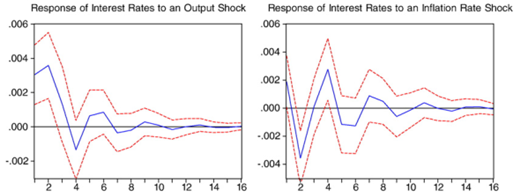
\includegraphics[width=\textwidth,height=0.4\textheight]{"C:/Users/Harriet/Documents/Econometrics/TimeSeriesProject/TimeSeriesProject/IRF_thirdclearmonetary.png"}

Cologni \& Manera found that the cointegrating vector for the US showed
a non-significant coefficient on the money demand variable and in the
long-run, this country shows an excess-output relationship and a
long-run negative effected of oil prices on excess output. Find no
instantaneous effect of oil prices on real GDP growth. Interest rates do
not rise due to inflation rate shock. United States IRFs are showing
that output significantly influenced by the oil shock. Monetary policy
impulse response is output shock and inflation shock. Found exchange
rates generally significantly impacted by oil price.

an increase in short-term interest rates results in a temporary decrease
in output, which peaks about four/five quarters after the initial
monetary policy shock and reverts back to the baseline level thereafter.
At the same time, inflation rate adjusts gradually downward. In Canada
and the U.S. the monetary contraction begins to affect output and real
money balances only after three or four quarters. In short, our results
suggest a temporary impact of monetary policy shocks on output and
inflation rate

Cointegrating vectors visually??

\ldots Let us see if we can impose the restrictions contained in the B
matrix onto the cointegrating vectors contained in the Et matrix.

\begin{verbatim}
## #############
## ###Model VECM 
## #############
## Full sample size: 108    End sample size: 104
## Number of variables: 6   Number of estimated slope parameters 126
## AIC -3210.216    BIC -2855.868   SSR 74.89496
## Cointegrating vector (estimated by ML):
##    realGDP worldoilprice interestrate   inflation exchangerate
## r1       1             0   -0.1704922 -0.01710960    0.6161332
## r2       0             1    1.6056301  0.06991751   -5.4962156
##    monetaryaggregate
## r1        -0.3747751
## r2         6.5786487
## 
## 
##                            ECT1                ECT2               
## Equation realGDP           0.0114(0.0262)      0.0012(0.0029)     
## Equation worldoilprice     -1.1213(0.6892)     -0.1191(0.0757)    
## Equation interestrate      -0.8253(1.3364)     -0.0909(0.1468)    
## Equation inflation         1.9807(4.2269)      0.2323(0.4642)     
## Equation exchangerate      -1.5280(0.4970)**   -0.1498(0.0546)**  
## Equation monetaryaggregate -0.0999(0.0543).    -0.0127(0.0060)*   
##                            Intercept             realGDP -1          
## Equation realGDP           -0.2387(0.5689)       0.3017(0.1198)*     
## Equation worldoilprice     23.9522(14.9378)      6.0850(3.1445).     
## Equation interestrate      18.0500(28.9642)      9.3757(6.0972)      
## Equation inflation         -43.1723(91.6115)     23.9182(19.2849)    
## Equation exchangerate      31.3052(10.7722)**    0.0695(2.2676)      
## Equation monetaryaggregate 2.3668(1.1764)*       -0.2741(0.2476)     
##                            worldoilprice -1    interestrate -1    
## Equation realGDP           -0.0015(0.0061)     -0.0022(0.0021)    
## Equation worldoilprice     0.4921(0.1589)**    -0.0330(0.0553)    
## Equation interestrate      0.5017(0.3081)      0.5658(0.1072)***  
## Equation inflation         4.0209(0.9746)***   -0.8458(0.3391)*   
## Equation exchangerate      0.3216(0.1146)**    0.0338(0.0399)     
## Equation monetaryaggregate -0.0342(0.0125)**   0.0027(0.0044)     
##                            inflation -1        exchangerate -1    
## Equation realGDP           -0.0007(0.0010)     0.0030(0.0035)     
## Equation worldoilprice     -0.0649(0.0261)*    0.0232(0.0930)     
## Equation interestrate      -0.1333(0.0505)**   -0.0459(0.1802)    
## Equation inflation         -0.3031(0.1598).    0.2740(0.5701)     
## Equation exchangerate      -0.0376(0.0188)*    -0.2884(0.0670)*** 
## Equation monetaryaggregate 0.0093(0.0021)***   -0.0107(0.0073)    
##                            monetaryaggregate -1 realGDP -2           
## Equation realGDP           -0.0421(0.0628)      0.2444(0.1211)*      
## Equation worldoilprice     -0.5255(1.6486)      1.0297(3.1793)       
## Equation interestrate      -0.7766(3.1966)      -0.0562(6.1646)      
## Equation inflation         1.3461(10.1107)      -10.4541(19.4983)    
## Equation exchangerate      -0.3822(1.1889)      -5.2154(2.2927)*     
## Equation monetaryaggregate 0.3084(0.1298)*      -0.4686(0.2504).     
##                            worldoilprice -2    interestrate -2   
## Equation realGDP           0.0033(0.0061)      0.0020(0.0025)    
## Equation worldoilprice     0.0529(0.1609)      0.0008(0.0653)    
## Equation interestrate      -0.3103(0.3121)     0.0588(0.1266)    
## Equation inflation         0.8367(0.9870)      0.1164(0.4004)    
## Equation exchangerate      0.0028(0.1161)      0.0796(0.0471).   
## Equation monetaryaggregate -0.0030(0.0127)     0.0014(0.0051)    
##                            inflation -2        exchangerate -2    
## Equation realGDP           -0.0010(0.0010)     -0.0023(0.0034)    
## Equation worldoilprice     -0.0211(0.0266)     -0.0957(0.0890)    
## Equation interestrate      0.0222(0.0516)      -0.1919(0.1725)    
## Equation inflation         -0.1823(0.1633)     -0.6758(0.5456)    
## Equation exchangerate      -0.0071(0.0192)     -0.1283(0.0642)*   
## Equation monetaryaggregate 0.0023(0.0021)      -0.0097(0.0070)    
##                            monetaryaggregate -2 realGDP -3          
## Equation realGDP           0.0925(0.0628)       -0.0572(0.1260)     
## Equation worldoilprice     2.1871(1.6496)       -1.6558(3.3091)     
## Equation interestrate      4.6408(3.1985)       5.5340(6.4163)      
## Equation inflation         4.7544(10.1165)      -8.8125(20.2941)    
## Equation exchangerate      0.7138(1.1896)       -10.8377(2.3863)*** 
## Equation monetaryaggregate -0.0451(0.1299)      0.2839(0.2606)      
##                            worldoilprice -3   interestrate -3    
## Equation realGDP           0.0061(0.0059)     0.0007(0.0022)     
## Equation worldoilprice     0.2848(0.1541).    0.0895(0.0570)     
## Equation interestrate      1.2330(0.2988)***  0.0649(0.1105)     
## Equation inflation         0.4219(0.9450)     0.9330(0.3494)**   
## Equation exchangerate      0.3740(0.1111)**   -0.0451(0.0411)    
## Equation monetaryaggregate -0.0218(0.0121).   -0.0080(0.0045).   
##                            inflation -3        exchangerate -3    
## Equation realGDP           -0.0016(0.0010)     0.0017(0.0034)     
## Equation worldoilprice     -0.0329(0.0258)     -0.0271(0.0888)    
## Equation interestrate      -0.1358(0.0500)**   -0.0992(0.1721)    
## Equation inflation         -0.0726(0.1580)     -0.5133(0.5445)    
## Equation exchangerate      -0.1181(0.0186)***  -0.0048(0.0640)    
## Equation monetaryaggregate 0.0050(0.0020)*     -0.0079(0.0070)    
##                            monetaryaggregate -3
## Equation realGDP           -0.0568(0.0583)     
## Equation worldoilprice     -0.4480(1.5304)     
## Equation interestrate      1.7129(2.9674)      
## Equation inflation         -1.4109(9.3857)     
## Equation exchangerate      3.0424(1.1036)**    
## Equation monetaryaggregate 0.0729(0.1205)
\end{verbatim}

\#Find VECM residuals

We want to compare our estimates to the one in Table 3.

Maybe instead it is the VAR system \ldots missing constant and trend

Then test for white noise residuals.

\hypertarget{step-6-is-it-stationary}{%
\section{Step 6: Is it stationary?}\label{step-6-is-it-stationary}}

\hypertarget{step-7-are-the-residuals-white-noise}{%
\section{Step 7: Are the residuals white
noise?}\label{step-7-are-the-residuals-white-noise}}

\hypertarget{step-8-find-vecm-model-by-imposing-sr-contemporaneous-effects}{%
\section{Step 8: Find VECM model by imposing SR contemporaneous
effects}\label{step-8-find-vecm-model-by-imposing-sr-contemporaneous-effects}}

\hypertarget{step-9-test-model-specification-using-congruency-parsimony-lag-inclusion}{%
\section{Step 9: Test model specification using congruency, parsimony,
lag
inclusion\ldots{}}\label{step-9-test-model-specification-using-congruency-parsimony-lag-inclusion}}

Alternatively, exclude exchange rates as the paper unusually included
these. However, in our models we could not find exchange rates to be
significant.

\hypertarget{appendix}{%
\section*{Appendix}\label{appendix}}
\addcontentsline{toc}{section}{Appendix}

\bibliography{Tex/ref}





\end{document}
